% Inspired by this video: youtube.com/watch?v=gG62zay3kck

\documentclass[aspectratio=169]{beamer}

\usepackage[T1]{fontenc}
\usepackage[utf8]{inputenc}

\usepackage[sfdefault,light]{FiraSans}

\usepackage{tikzducks}
\usepackage{graphicx}

\setbeamertemplate{navigation symbols}{}

\begin{document}
\pagestyle{empty}

\begin{frame}{}
\centering\Huge

Rhabarberbarbara

\end{frame}

\begin{frame}{}

\hspace{4.5cm}
\begin{tikzpicture}[scale=2]
\duck[
  longhair,
  tshirt=cyan,
  hat=blue
]
\end{tikzpicture}

\end{frame}

\begin{frame}{}

\hspace{4.5cm}
\begin{tikzpicture}[scale=2]
\duck[
  longhair,
  tshirt=cyan,
  hat=blue
]
\end{tikzpicture}

\begin{tikzpicture}[overlay]
\node at (10,4) {\LARGE Barbara};
\end{tikzpicture}

\end{frame}

\begin{frame}{}

\hspace{4.5cm}\begin{tikzpicture}[scale=2]
\duck[
  longhair,
  tshirt=cyan,
  hat=blue
]

\node[xshift=-10] at (wing) {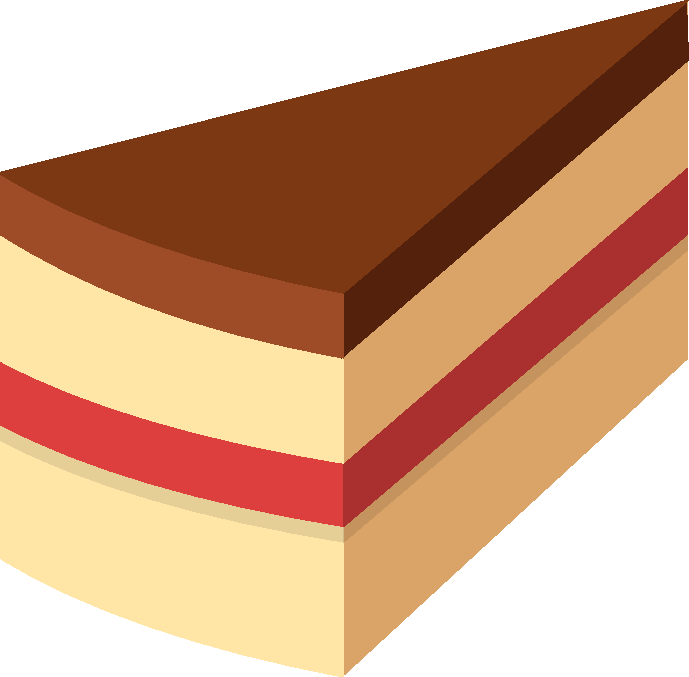
\includegraphics[scale=.1]{assets/cake}};
\end{tikzpicture}

\begin{tikzpicture}[overlay]
\node at (2.2,4) {\LARGE Rhabarberkuchen};
\end{tikzpicture}

\end{frame}

\begin{frame}{}

\hspace{4.5cm}\begin{tikzpicture}[scale=2]
\duck[
  longhair,
  tshirt=cyan,
  hat=blue
]

\node[xshift=-10] at (wing) {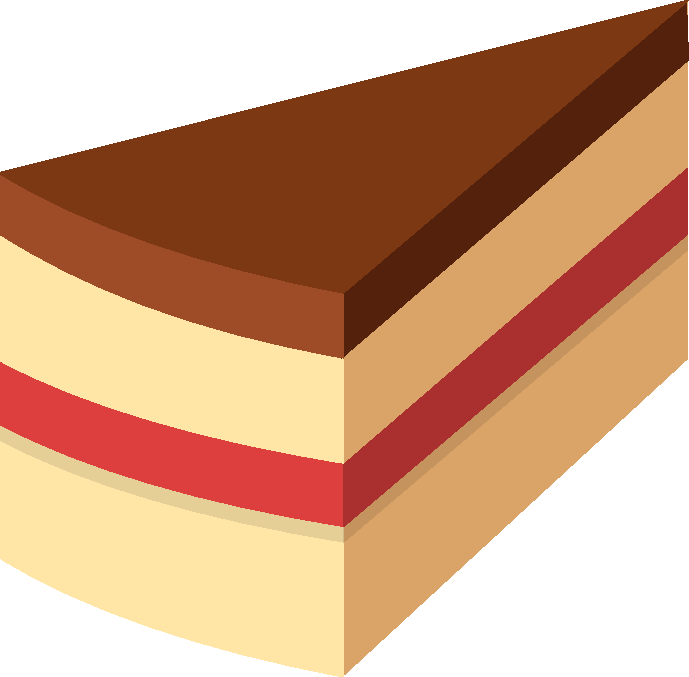
\includegraphics[scale=.1]{assets/cake}};
\end{tikzpicture}

\begin{tikzpicture}[overlay]
\node at (6.5,-0.5) {\LARGE Rhabarberbarbara};
\end{tikzpicture}

\end{frame}

\begin{frame}{}

\vspace*{-1.01cm}

\hspace{4.5cm}\begin{tikzpicture}[scale=2]
\duck[
  longhair,
  tshirt=cyan,
  hat=blue,
  think={\Huge\$\$\$}
]

\node[xshift=-10] at (wing) {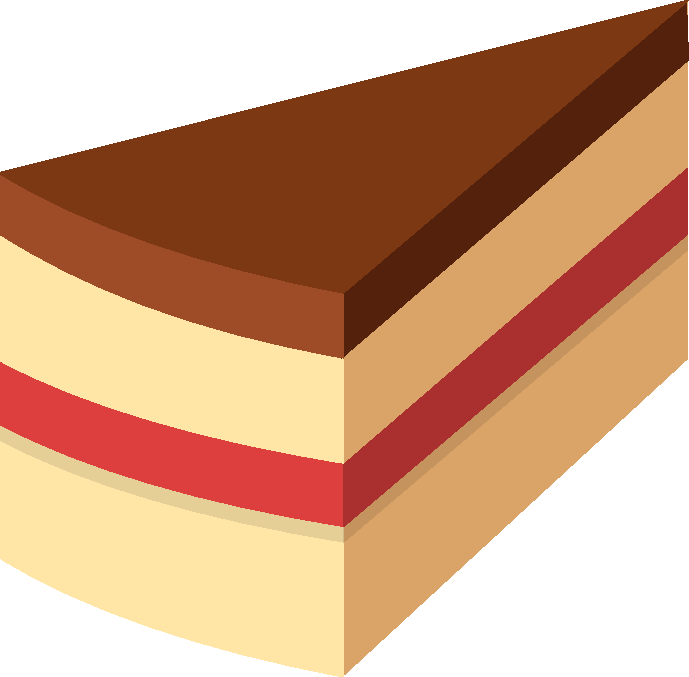
\includegraphics[scale=.1]{assets/cake}};
\end{tikzpicture}

\end{frame}

\begin{frame}{}

\hspace{3cm}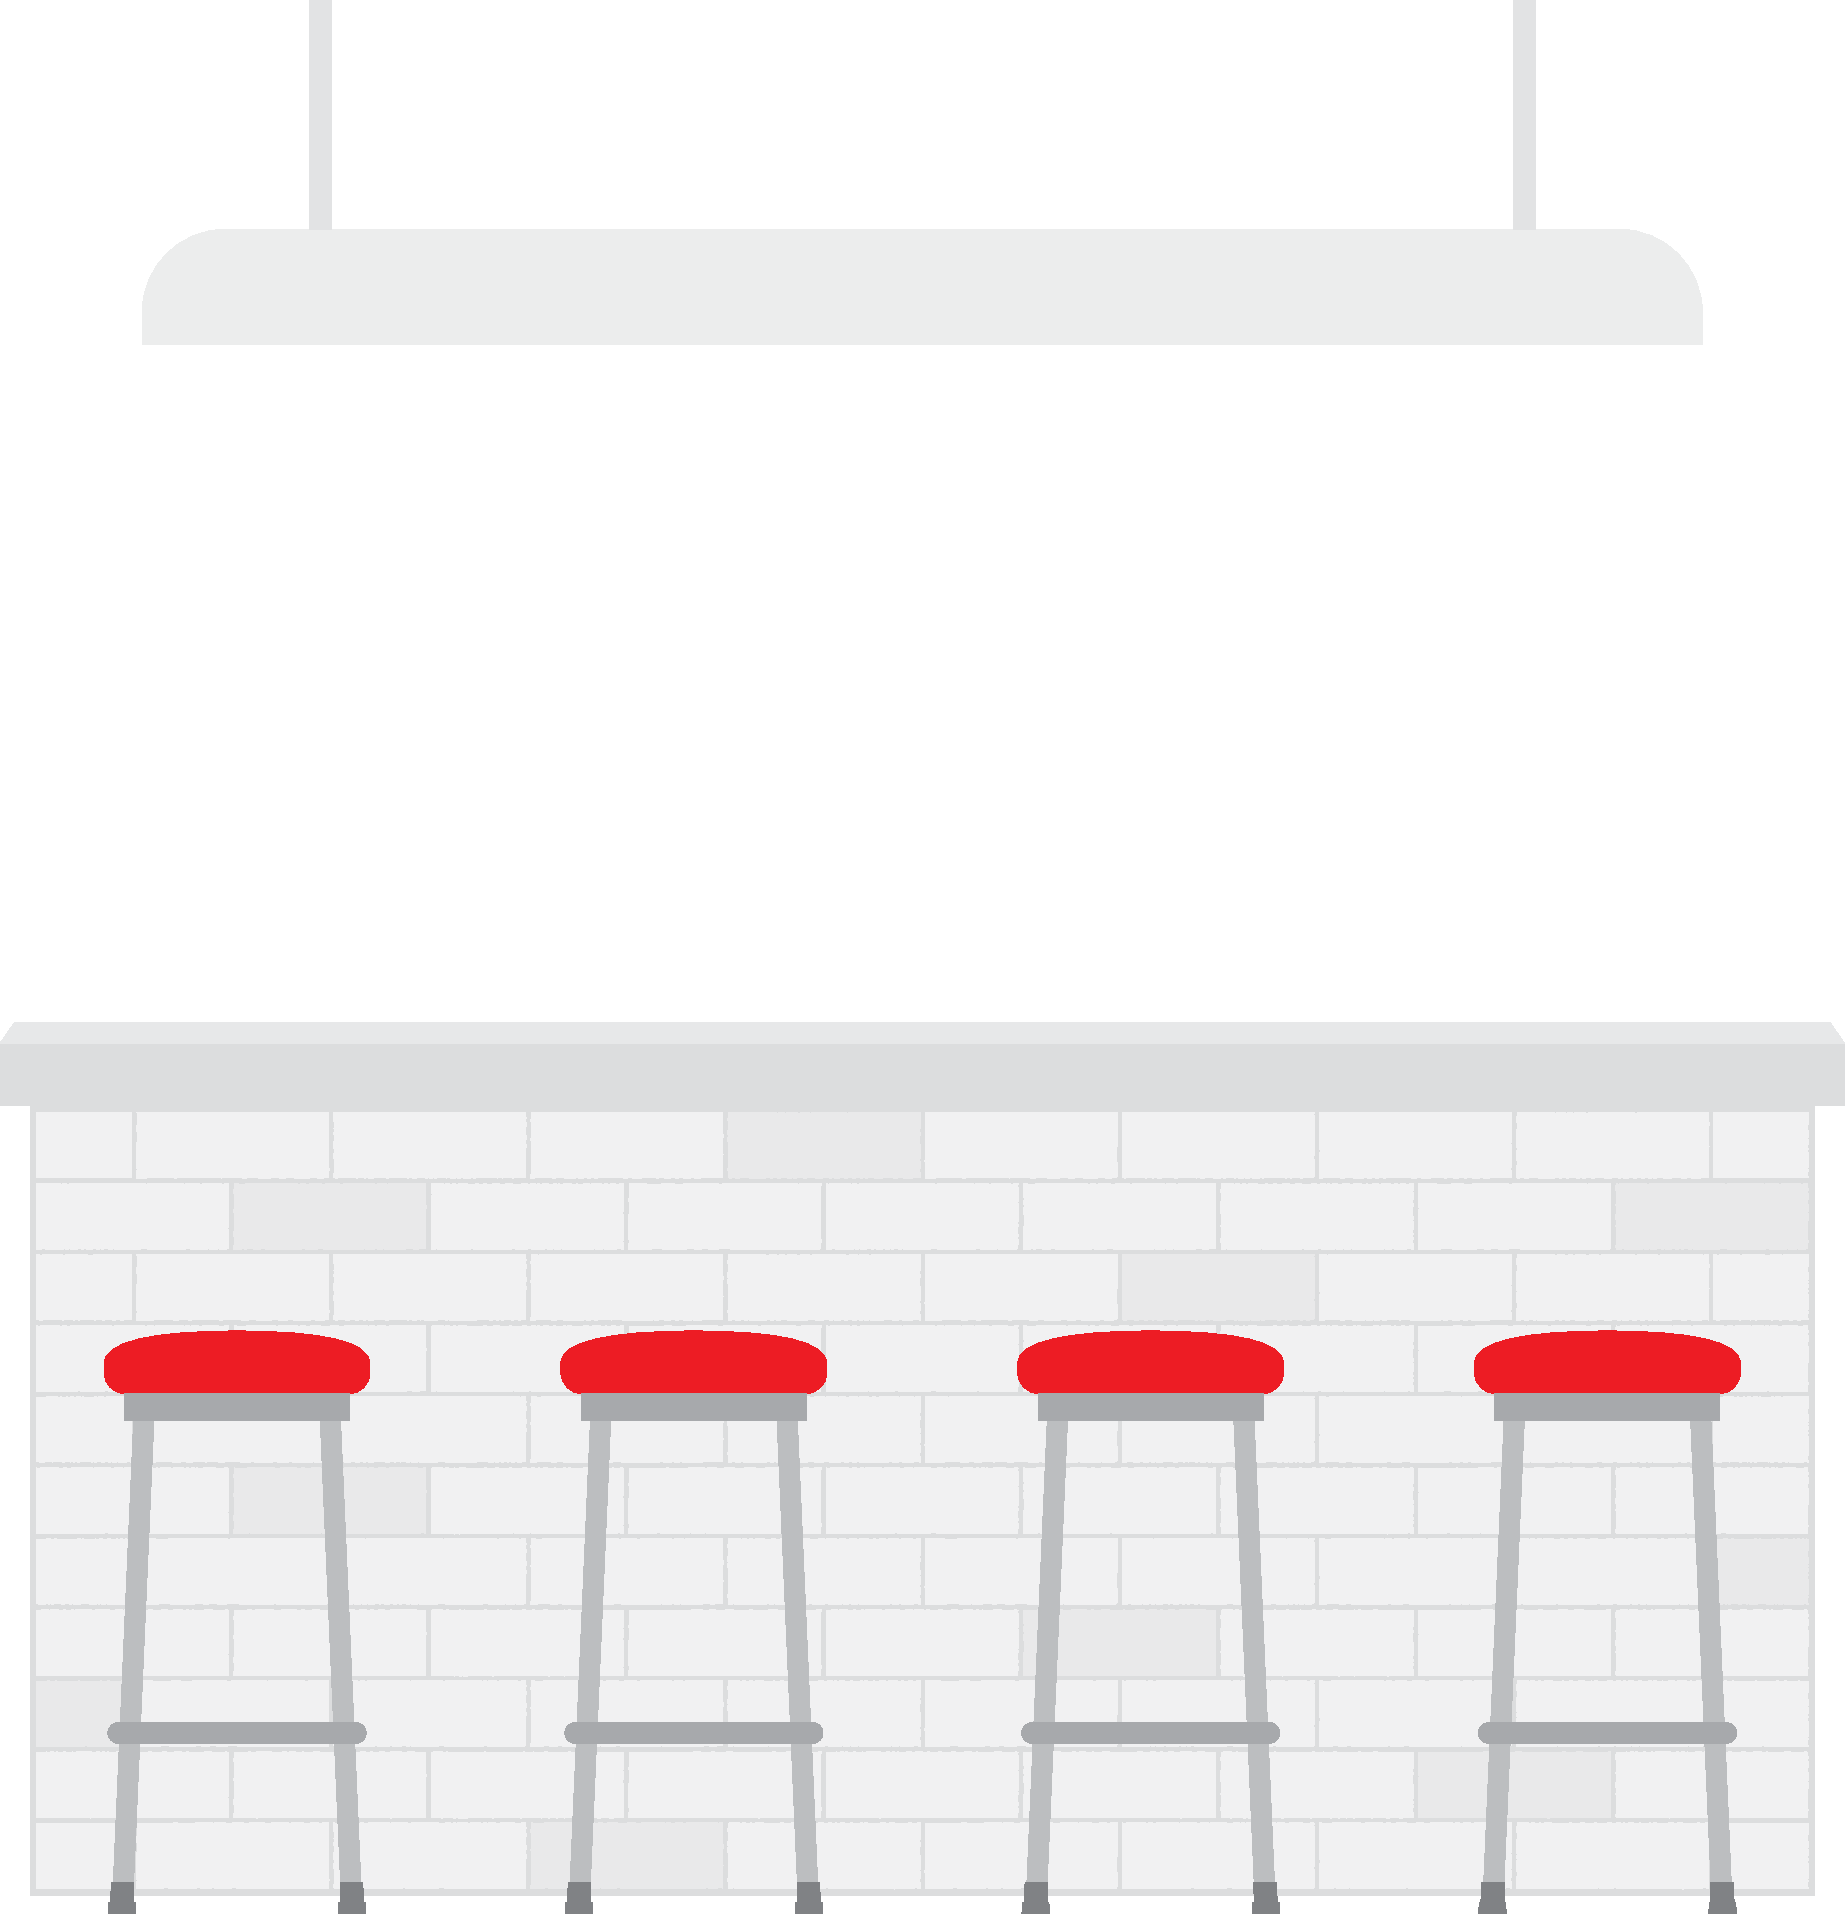
\includegraphics[scale=.25]{assets/bar}

\end{frame}

\begin{frame}{}

\hspace{3cm}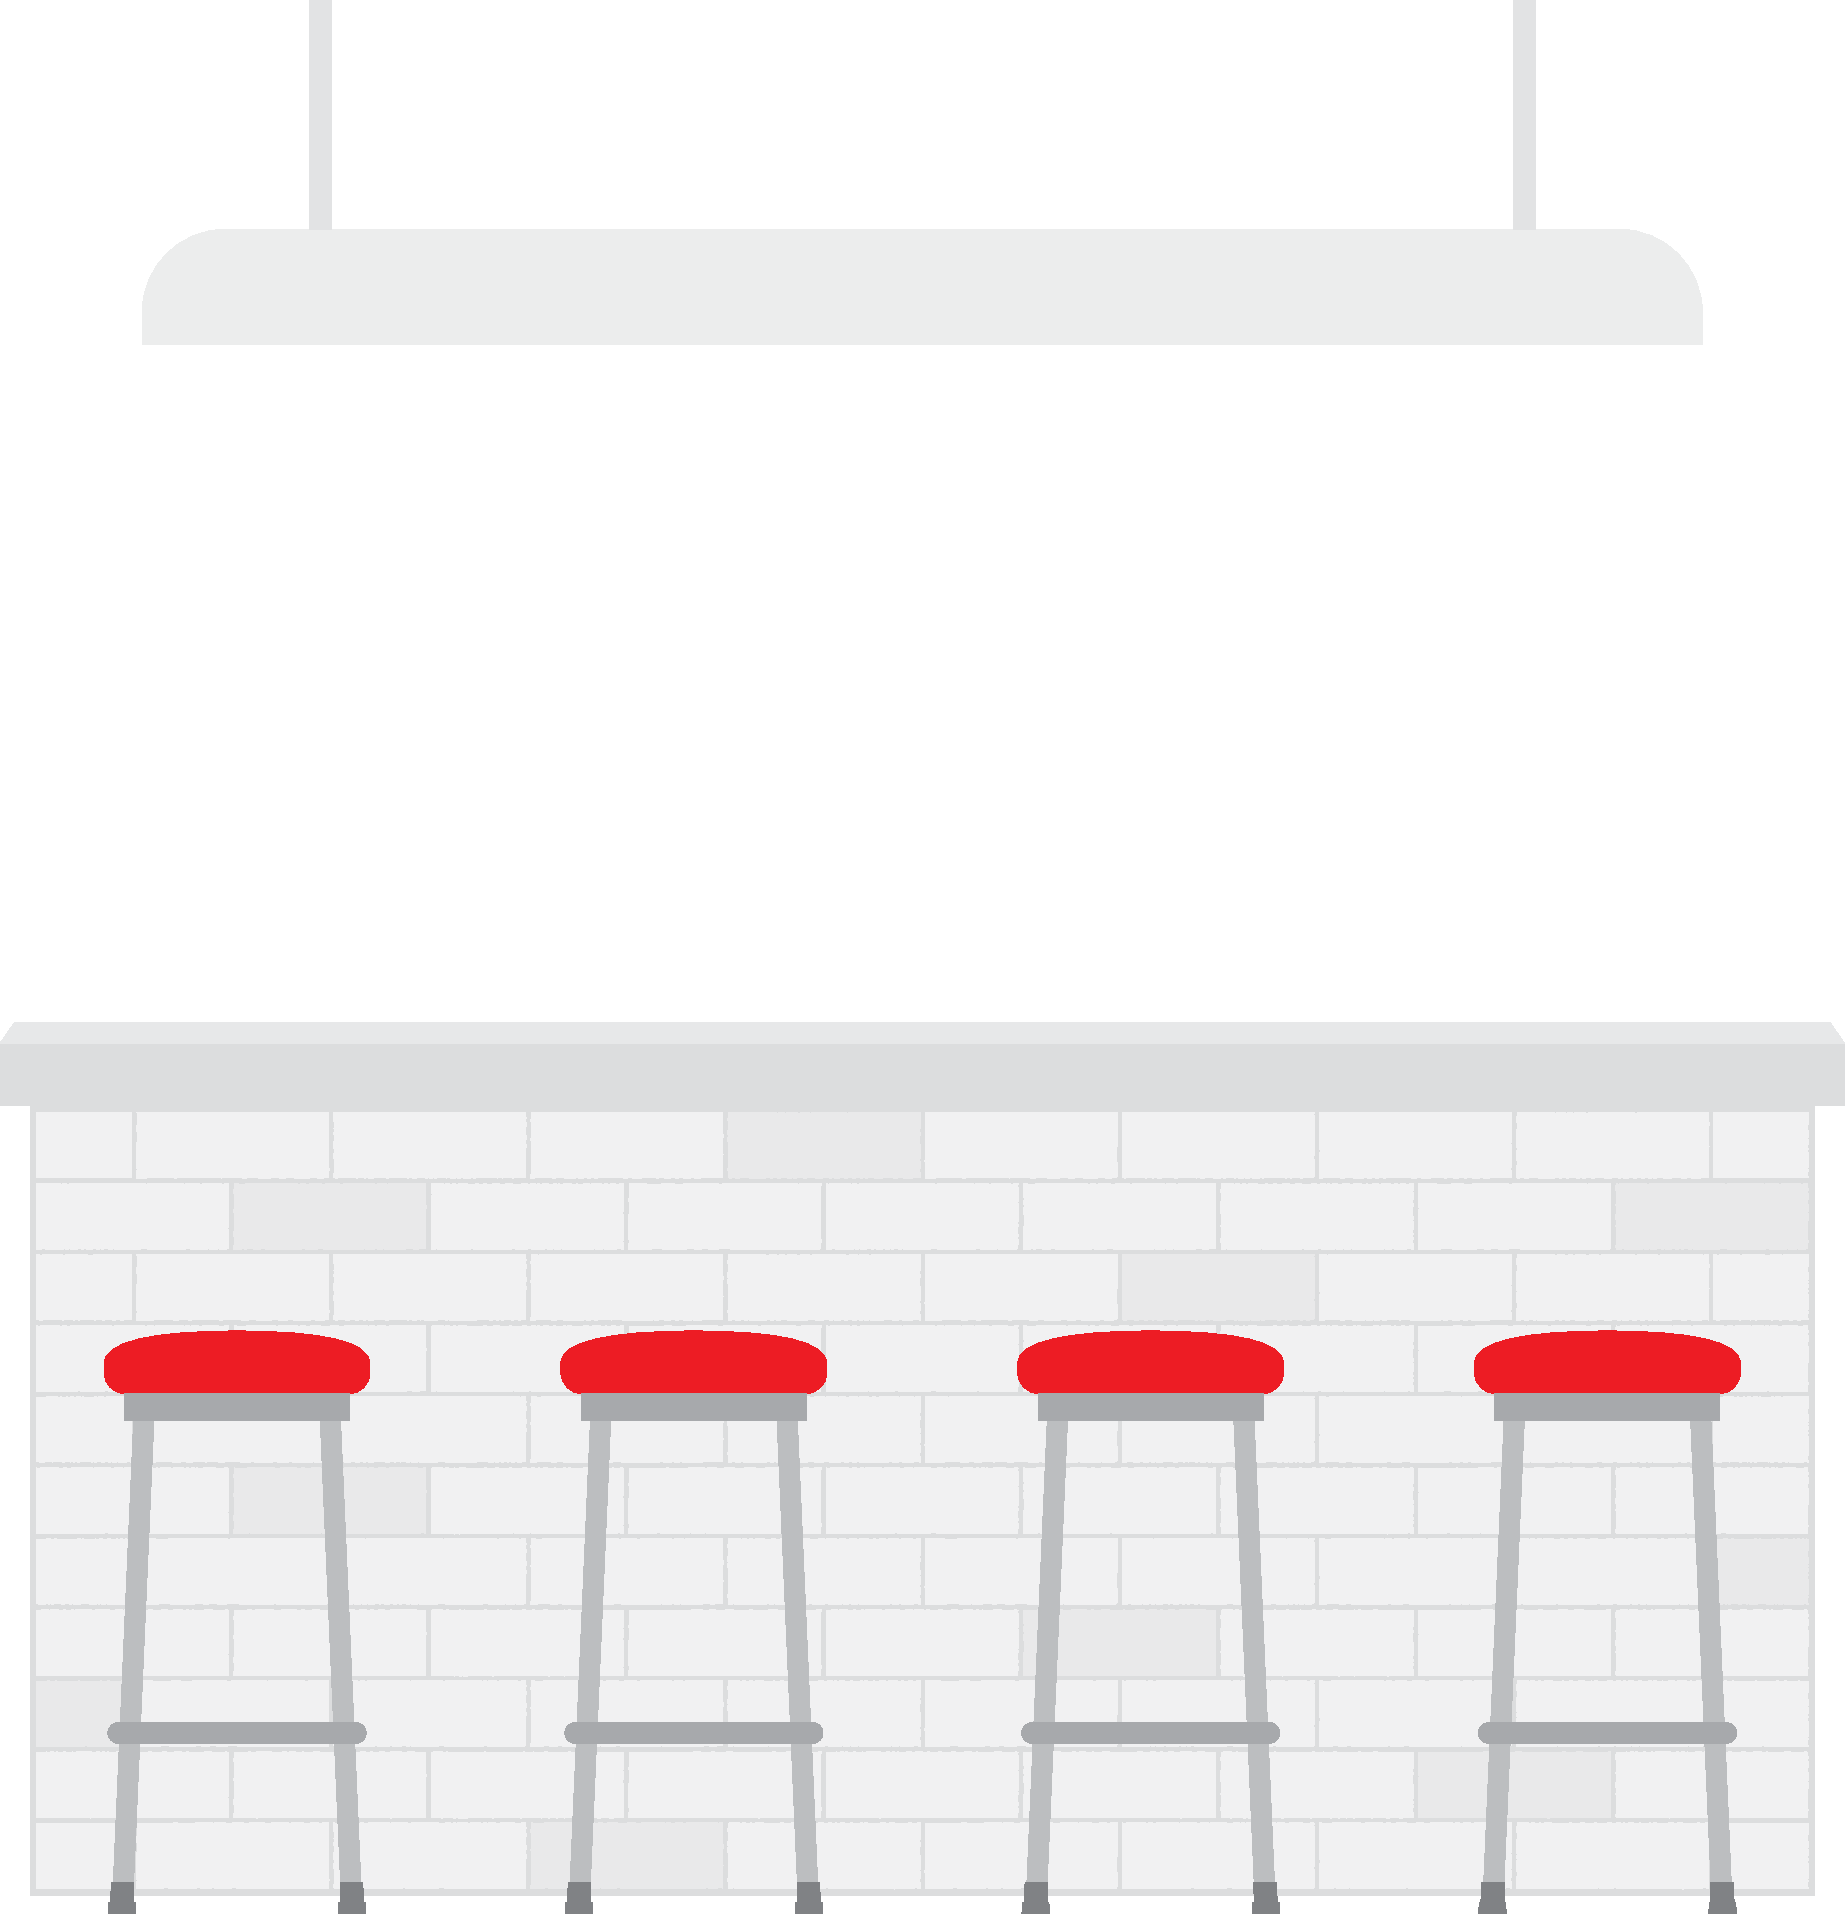
\includegraphics[scale=.25]{assets/bar}

\begin{tikzpicture}[overlay]
\node at (7,5) {\LARGE Rhabarberbarbarabar};
\end{tikzpicture}

\end{frame}

\begin{frame}{}

\hspace{4.5cm}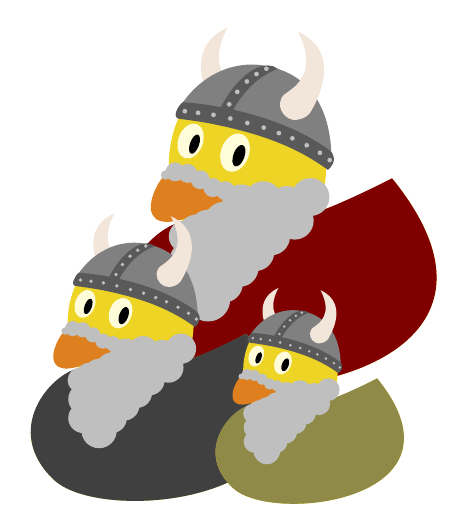
\begin{tikzpicture}[scale=2]
\duck[
  viking,
  tshirt=red!50!black,
  beard=gray!50!white
]

\duck[
  yshift=-20,
  scale=.8,
  xshift=-20,
  viking,
  tshirt=gray!50!black,
  beard=gray!50!white
]

\duck[
  yshift=-20,
  scale=.6,
  xshift=30,
  viking,
  tshirt=yellow!50!black,
  beard=gray!50!white
]
\end{tikzpicture}

\end{frame}

\begin{frame}{}

\hspace{4.5cm}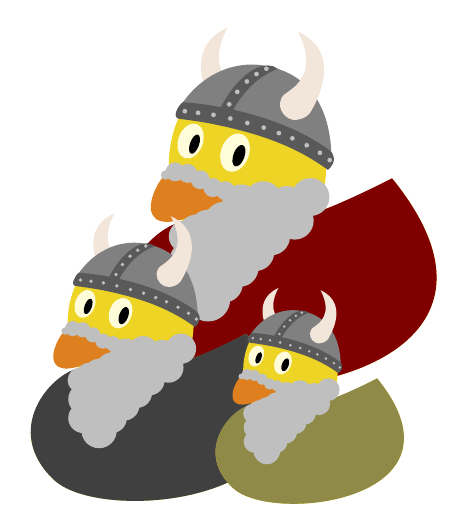
\begin{tikzpicture}[scale=2]
\duck[
  viking,
  tshirt=red!50!black,
  beard=gray!50!white
]

\duck[
  yshift=-20,
  scale=.8,
  xshift=-20,
  viking,
  tshirt=gray!50!black,
  beard=gray!50!white
]

\duck[
  yshift=-20,
  scale=.6,
  xshift=30,
  viking,
  tshirt=yellow!50!black,
  beard=gray!50!white
]
\end{tikzpicture}

\begin{tikzpicture}[overlay]
\node at (7,-0.5) {\LARGE Barbaren};
\end{tikzpicture}

\end{frame}

\begin{frame}{}

\hspace{3cm}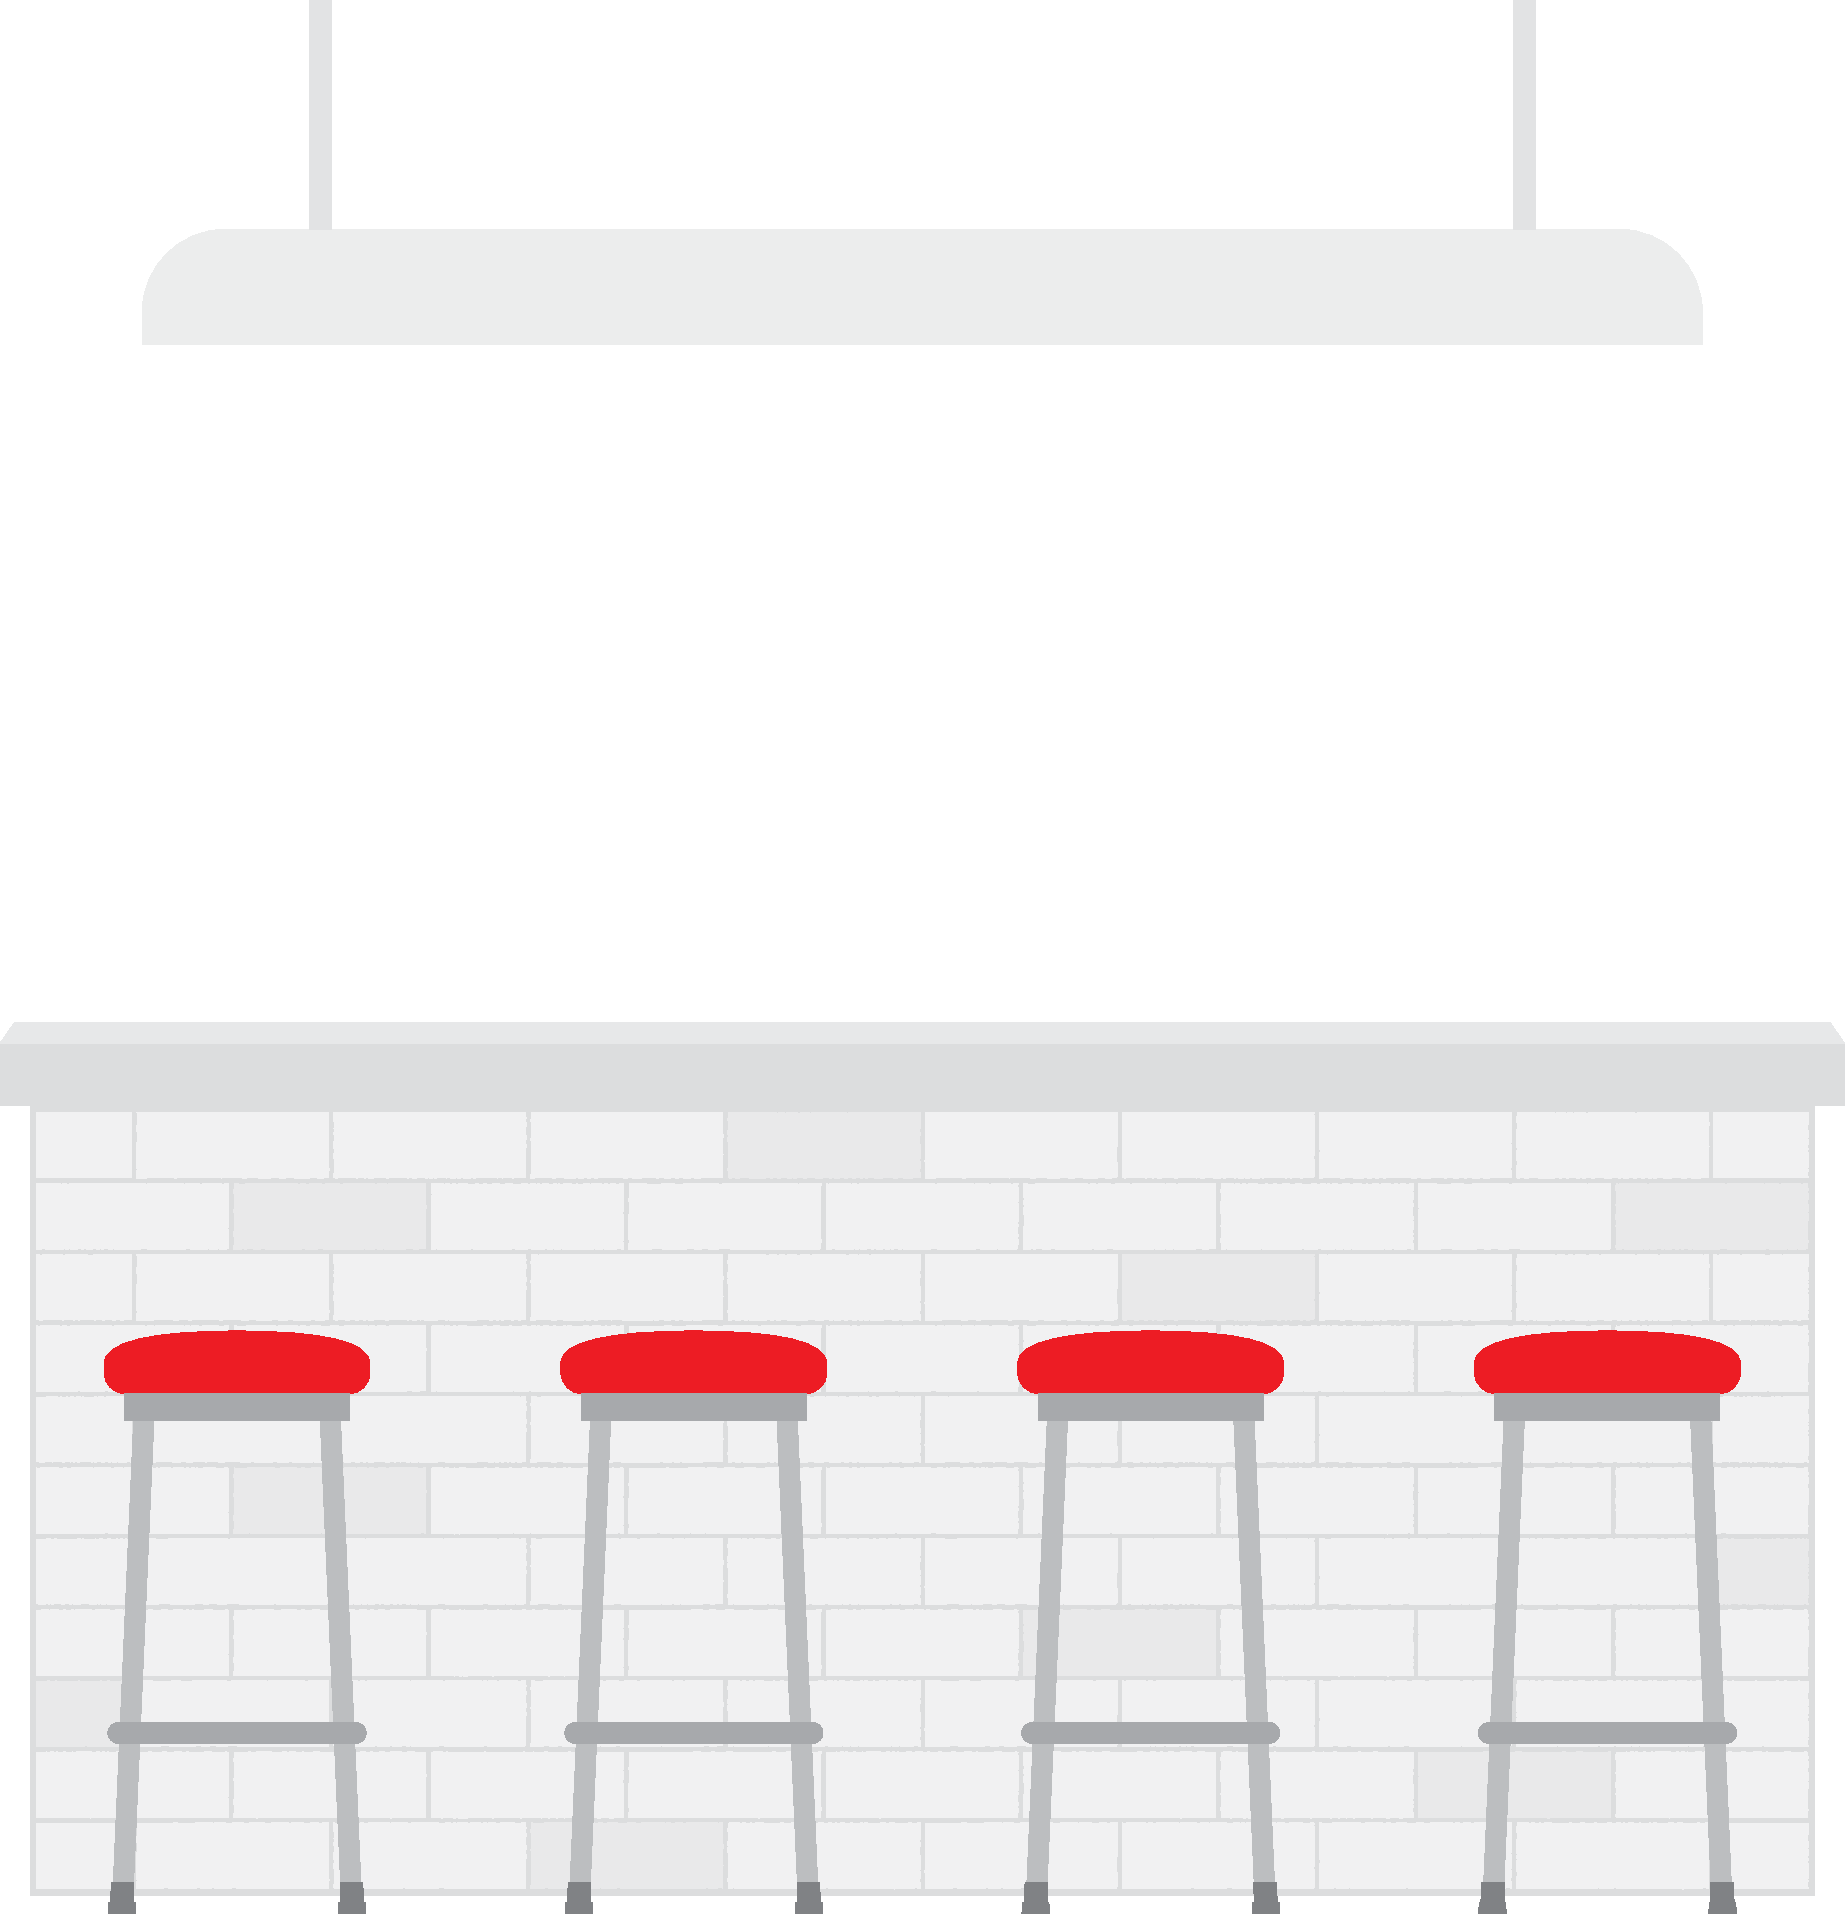
\includegraphics[scale=.25]{assets/bar}

\begin{tikzpicture}[overlay]
\node at (7,5) {\LARGE Rhabarberbarbarabar};
\end{tikzpicture}

\end{frame}

\begin{frame}{}

\hspace{4.5cm}\begin{tikzpicture}[scale=2]
\duck[
  longhair,
  tshirt=cyan,
  hat=blue
]

\node[xshift=-10] at (wing) {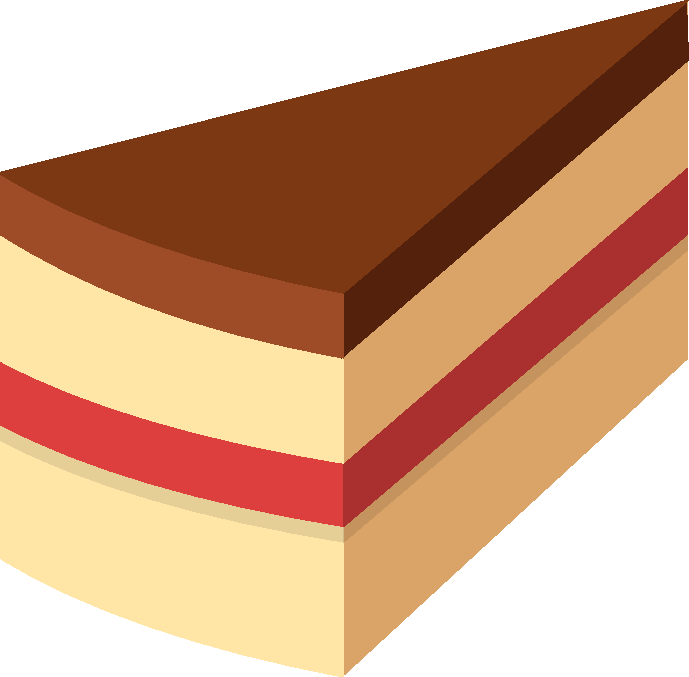
\includegraphics[scale=.1]{assets/cake}};
\end{tikzpicture}

\begin{tikzpicture}[overlay]
\node at (6.5,-0.5) {\LARGE Rhabarberbarbara};
\end{tikzpicture}

\end{frame}

\begin{frame}{}

\hspace{4.5cm}\begin{tikzpicture}[scale=2]
\duck[
  longhair,
  tshirt=cyan,
  hat=blue
]

\node[xshift=-10] at (wing) {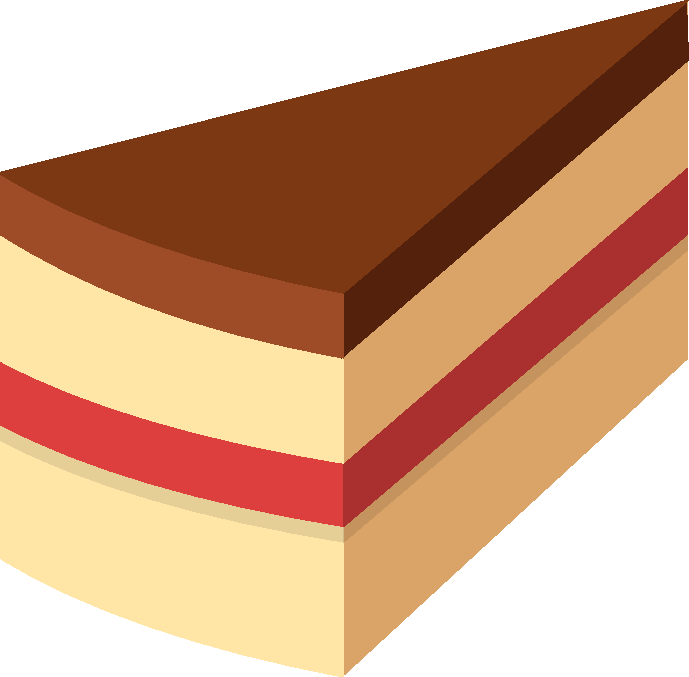
\includegraphics[scale=.1]{assets/cake}};
\end{tikzpicture}

\begin{tikzpicture}[overlay]
\node at (2.2,4) {\LARGE Rhabarberkuchen};
\end{tikzpicture}

\end{frame}

\begin{frame}{}

\hspace{4.5cm}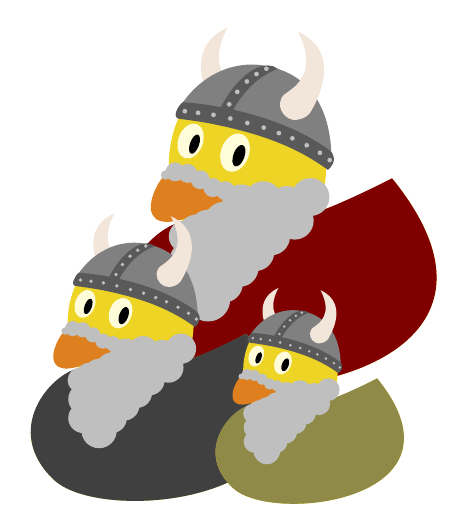
\begin{tikzpicture}[scale=2]
\duck[
  viking,
  tshirt=red!50!black,
  beard=gray!50!white
]

\duck[
  yshift=-20,
  scale=.8,
  xshift=-20,
  viking,
  tshirt=gray!50!black,
  beard=gray!50!white
]

\duck[
  yshift=-20,
  scale=.6,
  xshift=30,
  viking,
  tshirt=yellow!50!black,
  beard=gray!50!white
]
\end{tikzpicture}

\begin{tikzpicture}[overlay]
\node at (7,-0.5) {\LARGE Rhabarberbarbarabarbarbaren};
\end{tikzpicture}

\end{frame}

\begin{frame}{}

\hspace{4.5cm}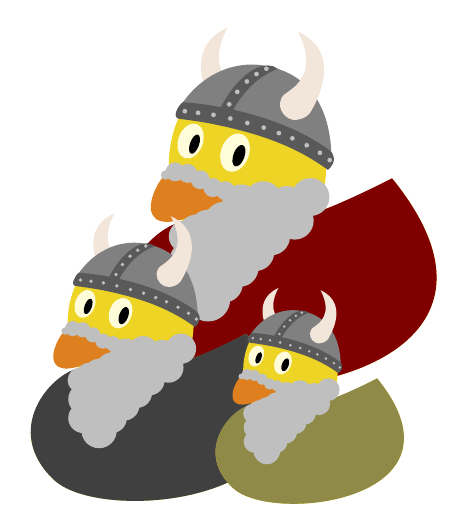
\begin{tikzpicture}[scale=2]
\duck[
  viking,
  tshirt=red!50!black,
  beard=gray!50!white
]

\duck[
  yshift=-20,
  scale=.8,
  xshift=-20,
  viking,
  tshirt=gray!50!black,
  beard=gray!50!white
]

\duck[
  yshift=-20,
  scale=.6,
  xshift=30,
  viking,
  tshirt=yellow!50!black,
  beard=gray!50!white
]
\end{tikzpicture}

\begin{tikzpicture}[overlay]
\node at (3.3,4) {\LARGE Bärte};
\end{tikzpicture}

\end{frame}

\begin{frame}{}

\hspace{4.5cm}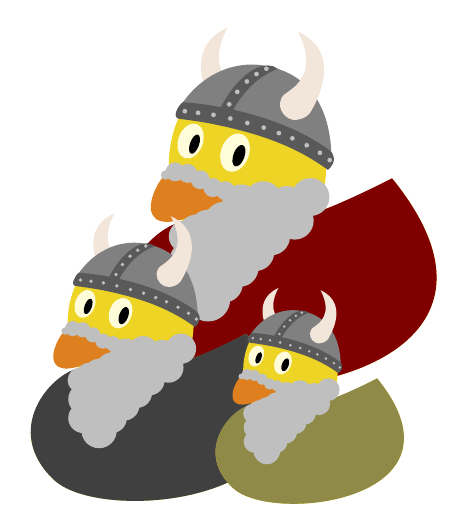
\begin{tikzpicture}[scale=2]
\duck[
  viking,
  tshirt=red!50!black,
  beard=gray!50!white
]

\duck[
  yshift=-20,
  scale=.8,
  xshift=-20,
  viking,
  tshirt=gray!50!black,
  beard=gray!50!white
]

\duck[
  yshift=-20,
  scale=.6,
  xshift=30,
  viking,
  tshirt=yellow!50!black,
  beard=gray!50!white
]
\end{tikzpicture}

\begin{tikzpicture}[overlay]
\node at (7,-0.5) {\LARGE Rhabarberbarbarabarbarbaren};
\end{tikzpicture}

\end{frame}

\begin{frame}{}

\hspace{4.5cm}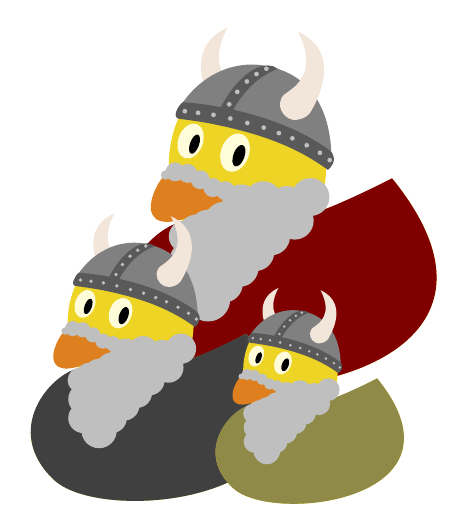
\begin{tikzpicture}[scale=2]
\duck[
  viking,
  tshirt=red!50!black,
  beard=gray!50!white
]

\duck[
  yshift=-20,
  scale=.8,
  xshift=-20,
  viking,
  tshirt=gray!50!black,
  beard=gray!50!white
]

\duck[
  yshift=-20,
  scale=.6,
  xshift=30,
  viking,
  tshirt=yellow!50!black,
  beard=gray!50!white
]
\end{tikzpicture}

\begin{tikzpicture}[overlay]
\node at (7,-0.5) {\LARGE Rhabarberbarbarabarbarbarenbart};
\end{tikzpicture}

\end{frame}

\begin{frame}{}

\hspace{6cm}\begin{tikzpicture}[scale=2]
\duck[
  shorthair=black,
  tshirt,
  jacket=gray,
  tie=cyan,
  glasses=red!50!black
]

\node[xshift=-30] at (wing) {
\includegraphics[scale=.3]{assets/scissors}};
\end{tikzpicture}

\begin{tikzpicture}[overlay]
\node at (11,4) {\LARGE Barbier};
\end{tikzpicture}

\end{frame}

% I STOPPED HERE

\begin{frame}{}

\vspace*{-.2cm}

\hspace{2.7cm}
\includegraphics[scale=.35]{assets/beer}
\hspace{1em}
\begin{tikzpicture}[scale=2]
\duck[
  shorthair=black,
  tshirt,
  jacket=gray,
  tie=cyan,
  glasses=red!50!black
]

\node[xshift=-30] at (wing) {
\includegraphics[scale=.3]{assets/scissors}};
\end{tikzpicture}

\end{frame}

\begin{frame}{}

\hspace{3cm}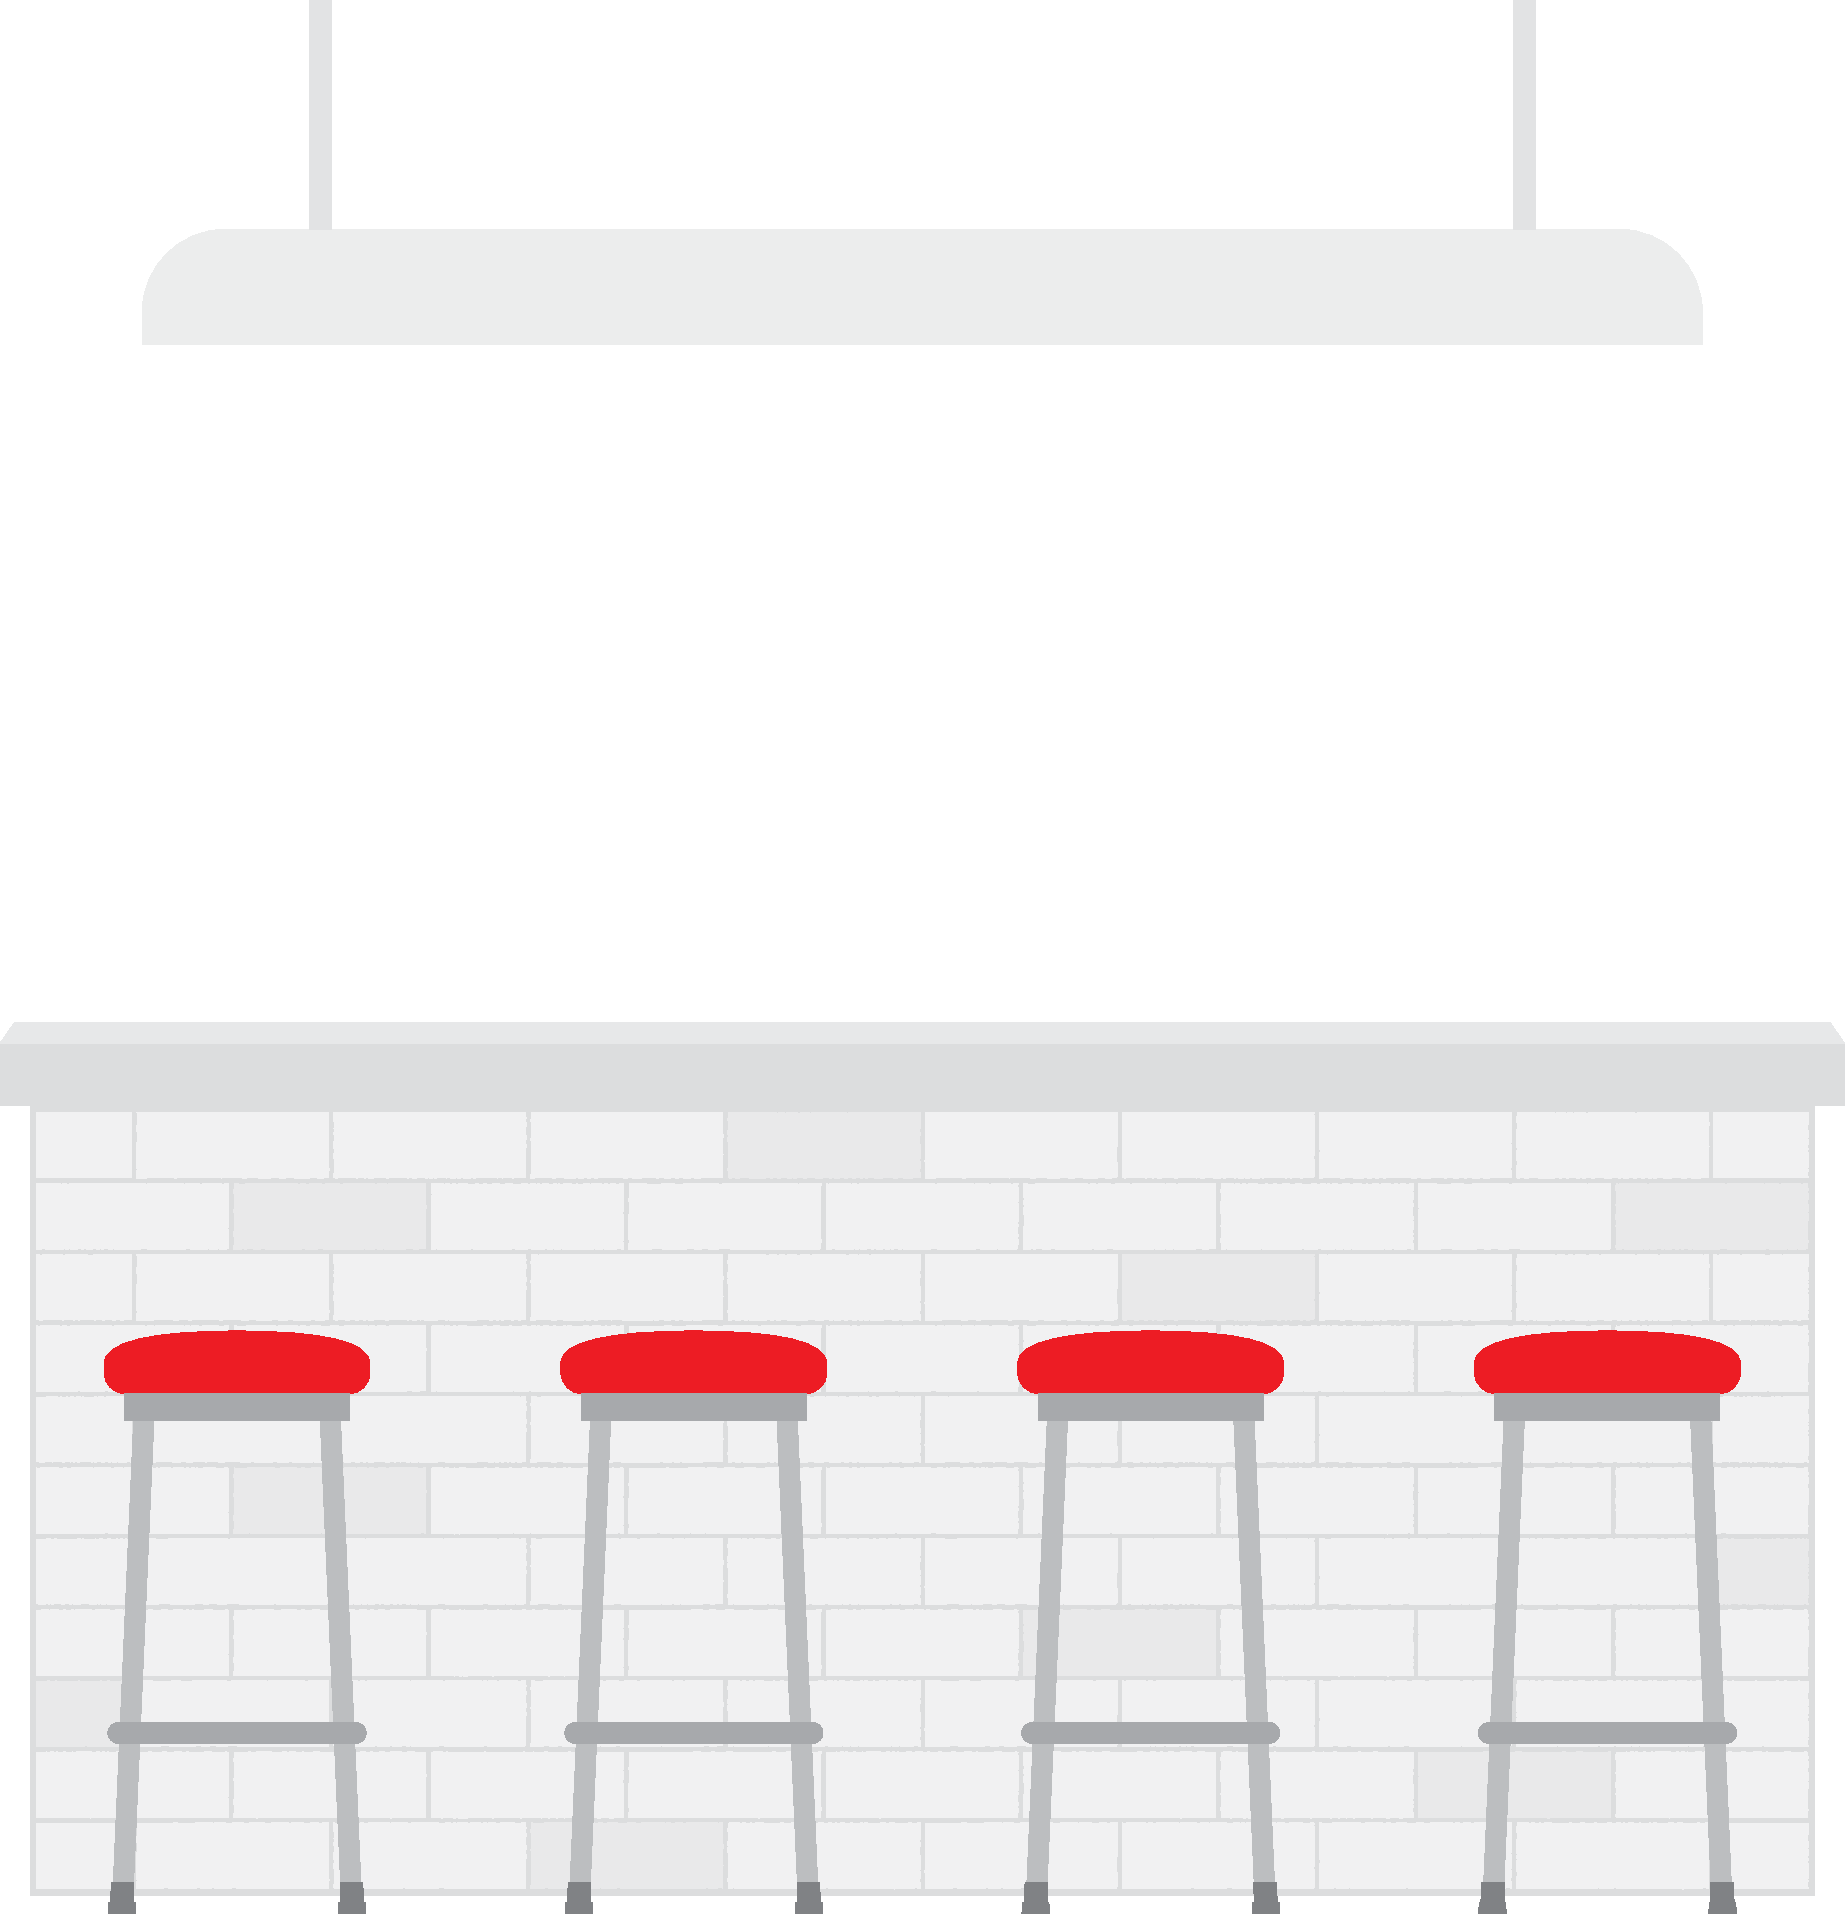
\includegraphics[scale=.25]{assets/bar}

\hspace{10cm}\begin{tikzpicture}[scale=1.5, overlay]
\duck[
  longhair=red!70!black,
  tshirt,
  jacket=gray!50!black,
  bowtie
]
\end{tikzpicture}

\end{frame}

\end{document}
